\documentclass{beamer}
\setbeamertemplate{section in toc}[sections numbered]
\usefonttheme[onlymath]{serif}
\beamertemplatenavigationsymbolsempty
\setbeamertemplate{footline}{% 
  \hfill% 
  \usebeamercolor[gray!50]{page number in head/foot}% 
  \usebeamerfont{page number in head/foot}% 
  \insertframenumber\,/\,\inserttotalframenumber%
}
\usepackage{amsmath}
\usepackage{graphicx}
\usepackage[tight,FIGTOPCAP]{subfigure}
\usepackage{lmodern}
\usepackage{amsmath}
\usepackage{braket}
\usepackage{color}
\usepackage{bm}
\usepackage{amssymb}
\usepackage{bbold}
\usepackage{tikz}
\usepackage{tikz-cd}
\usepackage{empheq}
\usepackage{caption}
\usepackage{stackengine}
\usepackage{framed}
\usepackage[percent]{overpic}
\usepackage{adjustbox}
\DeclareMathOperator{\sgn}{sgn}
\tikzset{>=latex}
\usetikzlibrary{matrix,calc,arrows,patterns,angles,quotes,shapes.geometric,positioning,decorations.pathreplacing,decorations.markings}
\newcommand{\blue}[1]{{\color{blue}{#1}}}
\newcommand{\ms}{\mathsf}
\renewcommand{\(}{\left(}
\renewcommand{\)}{\right)}
\renewcommand{\[}{\left[}
\renewcommand{\]}{\right]}
\tikzset{
  % style to apply some styles to each segment of a path
  on each segment/.style={
    decorate,
    decoration={
      show path construction,
      moveto code={},
      lineto code={
        \path [#1]
        (\tikzinputsegmentfirst) -- (\tikzinputsegmentlast);
      },
      curveto code={
        \path [#1] (\tikzinputsegmentfirst)
        .. controls
        (\tikzinputsegmentsupporta) and (\tikzinputsegmentsupportb)
        ..
        (\tikzinputsegmentlast);
      },
      closepath code={
        \path [#1]
        (\tikzinputsegmentfirst) -- (\tikzinputsegmentlast);
      },
    },
  },
  % style to add an arrow in the middle of a path
  mid arrow/.style={postaction={decorate,decoration={
        markings,
        mark=at position .5 with {\arrow[#1]{stealth}}
      }}},
}

%Information to be included in the title page:
\title{Chiral Dirac Superconductors: Second-order and Boundary-obstructed Topology}
%\author{Apoorv Tiwar, Ammar Jahin, and Yuxuan Wang}
%\institute{University of Florida}
\date{University of Florida, May 2020}

\begin{document}
\frame{\titlepage} 

\begin{frame}
    \frametitle{Recap of last time}
    \begin{itemize}
        \item The Dirac + ($p+ip$) model: $\mathcal{H}(\bm k) = f_1(\bm k) \sigma_x \tau_z + f_2(\bm k) \sigma_z \tau_z 
        + \Delta g_1(\bm k)  \tau_x + \Delta g_2(\bm k) \tau_y -\mu \tau_z$ \pause 
        \item In the topological phase the model looks like: 
        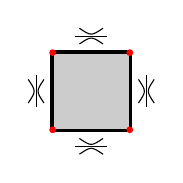
\begin{tikzpicture}[baseline=(O.base),scale=0.5]
            \node (O) at (0,-0.2) {};
            \draw[] (-0.4,1.4) -- (0.4,1.4);
            \draw[thin] (-0.3, 1.6) .. controls (0,1.4) .. (0.3,1.6);
            \draw[thin] (-0.3, 1.2) .. controls (0,1.4) .. (0.3,1.2);

            \draw[] (1.4,-0.4) -- (1.4,0.4);
            \draw[thin] (1.6, -0.3) .. controls (1.4,0) .. (1.6,0.3);
            \draw[thin] (1.2, -0.3) .. controls (1.4,0) .. (1.2,0.3);

            \draw[fill=black!20!white, draw=black, very thick] (-1,-1) rectangle (1,1);
            \draw[fill, red] (0.98,0.98) circle (2pt) (-0.98,0.98) circle (2pt) (0.98,-0.98) circle (2pt) (-0.98,-0.98) circle (2pt) ;

            \draw[] (-1.4,-0.4) -- (-1.4,0.4);
            \draw[thin] (-1.6, -0.3) .. controls (-1.4,0) .. (-1.6,0.3);
            \draw[thin] (-1.2, -0.3) .. controls (-1.4,0) .. (-1.2,0.3);

            \draw[] (-0.4,-1.4) -- (0.4,-1.4);
            \draw[thin] (-0.3, -1.6) .. controls (0,-1.4) .. (0.3,-1.6);
            \draw[thin] (-0.3, -1.2) .. controls (0,-1.4) .. (0.3,-1.2);
        \end{tikzpicture} \pause
        \item Discussed different phases for atomic insulators; obstructed atomic phases and the filling anomaly. \pause
        \item With $C_4$ symmetry (had we thought of the system as an insulator): 
        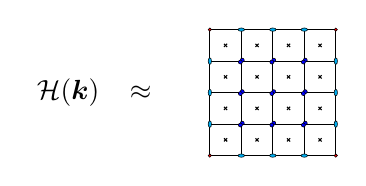
\begin{tikzpicture}[baseline=(O.base),scale = 0.4]
            \node[align=left] (O) at (-4.5,2) {$\mathcal{H}(\bm k)$};

            \node[align=left] at (-2.2,2) {$\approx$};

            \draw[black] (0,0) grid(4,4);

            \foreach \i in {0,...,3} 
            \foreach \j in {0,...,3} 
            {
            \draw[black] (\i+0.45,\j+0.45) -- (\i+0.55,\j+0.55);
            \draw[black] (\i+0.45,\j+0.55) -- (\i+0.55,\j+0.45);
            }
    
            \foreach \i in {1,...,3} 
            \foreach \j in {1,...,3} 
            {
            \draw[fill=blue, very thin] (\i+0.03 ,\j+0.03) circle (1.8pt);
            \draw[fill=blue, very thin] (\i-0.03 ,\j-0.03) circle (1.8pt);
            }
    
            \foreach \i in {1,...,3} 
            {
            \draw[fill=cyan, very thin] (0 ,\i ) ellipse (1.5pt and 3pt);
            \draw[fill=cyan, very thin] (4 ,\i ) circle (1.5pt and 3pt);
            \draw[fill=cyan, very thin] (\i ,0 ) circle (3pt and 1.5pt);
            \draw[fill=cyan, very thin] (\i ,4 ) circle (3pt and 1.5pt);
            }
            \draw[fill=red, very thin] (0 ,0 ) circle (1.5pt);
            \draw[fill=red, very thin] (4 ,0 ) circle (1.5pt);
            \draw[fill=red, very thin] (0 ,4 ) circle (1.5pt);
            \draw[fill=red, very thin] (4 ,4 ) circle (1.5pt);
        \end{tikzpicture}\pause
        \item Particle-hole symmetry implies that the corner charges of the obstructed atomic phase can be interpreted as Majorana zero modes for our BdG system. 
    \end{itemize}
\end{frame} 

\begin{frame}
    \frametitle{Outline}

    \begin{columns}
        \begin{column}{0.5\textwidth}
                \begin{table}
                    \centering
                    \def\arraystretch{0.4}
                    \begin{adjustbox}{width=\columnwidth,center}
                        \begin{tabular}{|| p{2.5cm}| p{2.5cm} | p{2.5cm}||} 
                        \hline
                        \begin{center} Model \end{center} 
                        &  \begin{center} With $C_{4}$ \end{center}   & \begin{center} With $C_{2}$  \end{center} \\ 
                        \hline\hline
                        \begin{center}
                        With PH
                        \end{center}
                        & %\rule{0pt}{4.6ex}
                        \begin{center}
                        HOTSC$_{2}$; \\
                        %\newline with 
                        corner Majorana 
                        %{\rule[-3.2ex]{0pt}{0pt}} 
                        \end{center}
                        & 
                        \begin{center}
                        BOTSC$_2$; \\
                        %\newline with 
                        corner Majorana 
                        \end{center}
                        \\ 
                        \hline
                        \begin{center}
                        Without PH
                        \end{center} &
                        \begin{center}
                        HOTI$_{2}$; \\
                        %\rule{0pt}{4.6ex}
                        % \newline with 
                        filling anomaly
                        % {\rule[-3.2ex]{0pt}{0pt}}
                        \end{center}
                        & 
                        \begin{center}
                        Trivial
                        \end{center}
                            \\ 
                        \hline
                        \end{tabular}
                \end{adjustbox}
            \end{table}
        \end{column}
        \begin{column}{0.5\textwidth}
            \begin{itemize}
                \item Understanding the corner mode from defect classification.
                \item Discuss the second column of the table. 
            \end{itemize}
        \end{column}
    \end{columns}

\end{frame}


\begin{frame}
    \frametitle{Defect classification}
    \begin{columns}
        \begin{column}{0.6\textwidth}
            \begin{itemize}
                \item Teo-Kane classification of defect Hamiltonians, $\mathcal{H}(\bm k,\bm r)$.
                \item $d$ is dimension of $\bm k$. $D$ is the dimension of $\bm r$.
                \item Depends on the symmetry class and the dimension of the defect.
            \end{itemize} 
        \end{column}
        \begin{column}{0.4\textwidth}
            \begin{figure}[]
                \centering
                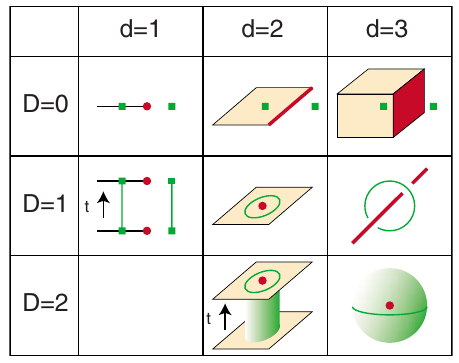
\includegraphics[scale=0.33]{teo-kane_defect_table.png}
            \end{figure}
        \end{column}
    \end{columns}

    \begin{overpic}[width=\textwidth]{defect_classification.png}
        
    \end{overpic}

\end{frame}

\begin{frame}
    \frametitle{Real space picture of the topological invariant}
    \begin{columns}
        \begin{column}{0.6\textwidth}
            \begin{itemize}
                \item The basic idea is to treat the corner of the sample as a defect, $\mathcal{H}(\bm k, \Phi)$.
                \item For class BDI the topological invariant corresponds to the number of Majorana modes bound to the corner.   
            \end{itemize}
        \end{column}
        \begin{column}{0.4\textwidth}
            \begin{figure}[]
                \centering
                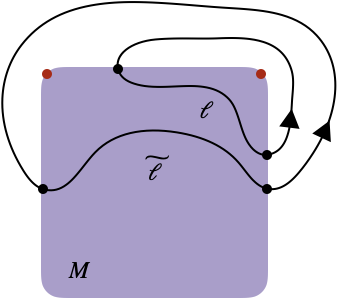
\includegraphics[scale=0.3]{Real_space_path.png}
            \end{figure}
        \end{column}
    \end{columns}
    \begin{overpic}[width=\textwidth]{defect_classification.png}
        \put (47.3,14.2) 
        {
            
\begin{tikzpicture}
                \draw[red, thick] (0,0) ellipse (5pt and 9pt);
            \end{tikzpicture}
        }
    \end{overpic}

\end{frame}

\begin{frame}
    \frametitle{Real space picture of the topological invariant}
    Model the outside by: 
    \begin{align*}
        \mathcal H_{\ms{triv}}(\bm{k})= -f_0(\sigma_x\tau_z + \sigma_z \tau_z) +\Delta \sin(k_x)\tau_x + \Delta \sin(k_y)\tau_y -\mu \tau_z
    \end{align*} \pause
    \begin{itemize}
        \item If our system with $\sgn(f_\Gamma)\sgn(f_M) = -1$ has $f_\Gamma = f_0$, then the physics of the system is completely determined by what happens near the $\Gamma$ point. 
    \end{itemize} \pause
    
    Define $\bm q$ to be a small momentum deviation from the $\Gamma$ point. The defect Hamiltonian near the $\Gamma$ point (for $\mu=0$): 
    \begin{columns}
        \begin{column}{0.6\textwidth}
            \begin{align*}
                &\mathcal H(\bm{q}+ \Phi)=\Delta q_{x}\tau_x + \Delta q_{y}\tau_y\\ 
                &\qquad + f_0 \left[ \cos (\Phi) \sigma_x \tau_z +\sin(\Phi) \sigma_z \tau_z \right] \\ 
                &\Phi = \pi/4 \rightarrow \text{inside material} \\ 
                &\Phi = 5\pi/4 \rightarrow \text{outside material}
            \end{align*}
            
        \end{column}
        \begin{column}{0.4\textwidth}
            \begin{figure}[]
                \centering
                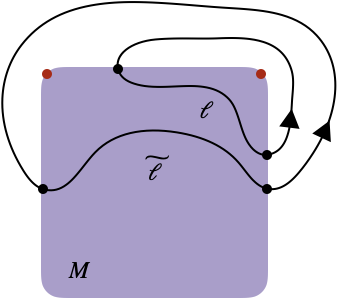
\includegraphics[scale=0.3]{Real_space_path.png}
            \end{figure}
        \end{column}
    \end{columns}

\end{frame}

\begin{frame}
    \frametitle{Real space picture of the topological invariant}
    \begin{columns}
        \begin{column}{0.6\textwidth}
            \begin{align*}
                \mathcal H(\bm{q},\Phi)&=\Delta q_{x}\tau_x + \Delta q_{y}\tau_y\\ &+ f_0 \left[ \cos (\Phi) \sigma_x \tau_z +\sin(\Phi) \sigma_z \tau_z \right]
            \end{align*}
            With $C_4$ symmetry it can be shown: 
            \begin{align*}
                \mathsf{N}_{\mathsf{w}}:=\frac{1}{2\pi}\oint_{\ell} \mathrm{d}\Phi = (2n + 1).
            \end{align*}
            Adding the Chemical potential reduces the $Z$ topological invariant to a $Z_2$. 
        \end{column}
        \begin{column}{0.4\textwidth}
            \begin{figure}[]
                \centering
                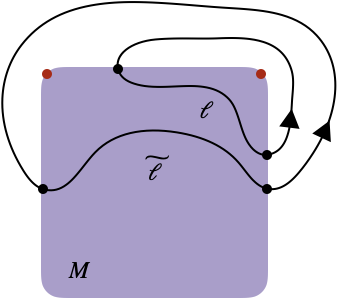
\includegraphics[scale=0.3]{Real_space_path.png}
            \end{figure}
        \end{column}
    \end{columns}

\end{frame}


\section{Boundary-obstructed topology}
\subsection{Dirac + \texorpdfstring{($p+ip$)}{} with \texorpdfstring{$\ms{C}_2$}{} symmetry}

\begin{frame}
    \frametitle{A cheap way of getting Majorana zero modes}
    Consider the following cheap way of getting Majorana zero modes on the corners: 
    \begin{columns}
        \begin{column}{0.4\textwidth}
            \begin{figure}[]
                \centering
                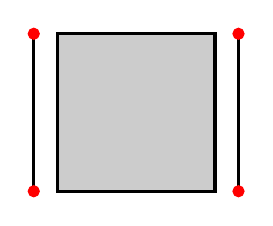
\begin{tikzpicture}
                    \draw[fill=black!20!white, draw=black, very thick] (-1,-1) rectangle (1,1);
                    \draw [black, very thick] (1.3,-1) -- (1.3,1);
                    \draw [fill,red] (1.3,-1) circle (2pt) (1.3,1) circle (2pt);
                    \draw [black, very thick] (-1.3,-1) -- (-1.3,1);
                    \draw [fill,red] (-1.3,-1) circle (2pt) (-1.3,1) circle (2pt);
                \end{tikzpicture}
            \end{figure}
        \end{column}\pause
        \begin{column}{0.6\textwidth}
            \begin{itemize}
                \item Not $C_4$ symmetric, relax $C_4$ to $C_2$.\pause
                \item Majorana zero modes can be removed without closing a bulk gap. \pause
                \item The edge gap become essential for capturing the topology of the system. 
            \end{itemize}
        \end{column}
    \end{columns}\pause
    \begin{framed}
        Such topological phases protected by an edge gap closing are called boundary obstructed topological phases.
    \end{framed}
\end{frame}
\begin{frame}
    \frametitle{The prototypical Hamiltonian as an example of BOTSC$_2$}
    Our prototypical model with only $C_2$ symmetry can at best be boundary obstructed. 
    \begin{columns}
        \begin{column}{0.45\textwidth}
            \begin{align*}
                \mathcal{H}(\bm k) &= (\gamma_x + \cos(k_x)) \tau_z \\ 
                & + (\gamma_y + \cos(k_y))\sigma_z \tau_z \\
                & +\Delta \sin(k_x) \tau_x \\
                & + \Delta \sin(k_y) \tau_y -\mu \tau_z,
            \end{align*} 
            Topological phase can be deformed into trivial phase without closing the bulk gap. 
            \visible<2->{
            \begin{framed}
                Need to study the edges carefully. 
            \end{framed}
            }
        \end{column}
        \begin{column}{0.55\textwidth}
            \begin{figure}[]
                \centering
                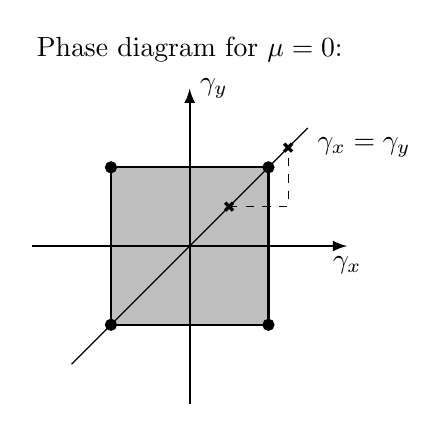
\begin{tikzpicture}
                    \node[align=center] at (0,2.5) {Phase diagram for $\mu=0$:};
                    \draw[fill=gray!50,draw=black, thick] (-1,-1) rectangle (1,1);
                    \draw[black] (-1.5,-1.5) -- (1.5,1.5) node[anchor=north west] {$\gamma_x = \gamma_y$};
                    \draw[fill, black] (-1,-1) circle (2pt) (1,-1) circle (2pt) (-1,1) circle (2pt) (1,1) circle (2pt);
                    \draw[thick,->] (-2,0) -- (2,0) node[anchor=north] {$\gamma_x$};
                    \draw[thick,->] (0,-2) -- (0,2) node[anchor=west] {$\gamma_y$};

                    \draw[black, very thick] (0.5 -0.05,0.5 -0.05) -- (0.5 + 0.05,0.5+0.05);
                    \draw[black, very thick] (0.5 - 0.05,0.5 + 0.05) -- (0.5 + 0.05,0.5 -0.05);

                    \draw[black, very thick] (1.25 -0.05,1.25 -0.05) -- (1.25 + 0.05,1.25+0.05);
                    \draw[black, very thick] (1.25 - 0.05,1.25 + 0.05) -- (1.25 + 0.05,1.25 -0.05);
                    \draw[black, dashed] (0.5,0.5) -- (1.25,0.5) -- (1.25,1.25); 
                \end{tikzpicture}
            \end{figure}
        \end{column}
    \end{columns}

\end{frame}

\begin{frame}
    \frametitle{Boundary obstructed atomic phases.} 
    Boundary obstruction protected by mirror symmetry: 
    \begin{figure}[]
        \subfigure{
        \centering
        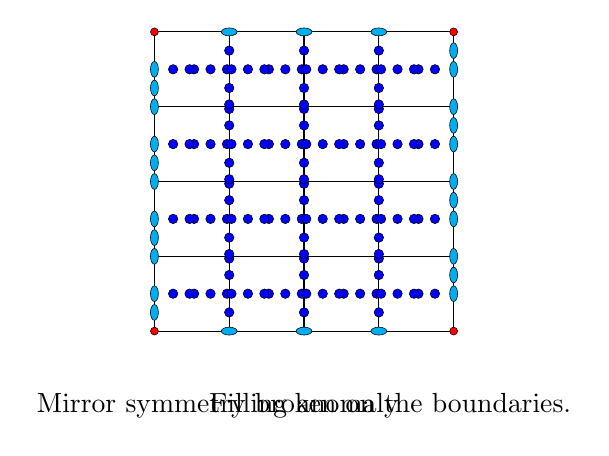
\begin{tikzpicture}[scale = 0.95]
            \draw[black] (0,0) grid(4,4);
    
            \foreach \i in {0,...,3} 
            \foreach \j in {0,...,3} 
            {
            \draw[black] (\i+0.45,\j+0.45) -- (\i+0.55,\j+0.55);
            \draw[black] (\i+0.45,\j+0.55) -- (\i+0.55,\j+0.45);
            }
            \visible<1>{
            \foreach \i in {0,...,3} 
            \foreach \j in {0,...,3} 
            {
            \draw[fill=blue, very thin] (\i+0.03+0.5 ,\j+0.5) circle (1.8pt);
            \draw[fill=blue, very thin] (\i-0.03+0.5 ,\j+0.5) circle (1.8pt);
            }
            }
            \visible<2>{
            \foreach \i in {0,...,3} 
            \foreach \j in {0,...,3} 
            {
            \draw[fill=blue, very thin] (\i+0.5+0.25 ,\j+0.5) circle (1.8pt);
            \draw[fill=blue, very thin] (\i+0.5-0.25 ,\j+0.5) circle (1.8pt);
            }
            }
            \visible<3>{
            \foreach \j in {0,...,3} 
            {
            \foreach \i in {0,...,2} 
            {
            \draw[fill=blue, very thin] (\i+0.97 ,\j+0.5) circle (1.8pt);
            }
            \draw[fill=cyan, very thin] (4, \j+0.5) ellipse (1.5pt and 3pt);
            }
            \foreach \j in {0,...,3} 
            {
            \foreach \i in {1,...,3} 
            {
            \draw[fill=blue, very thin] (\i+0.03 ,\j+0.5) circle (1.8pt);
            }
            \draw[fill=cyan, very thin] (0, \j+0.5) ellipse (1.5pt and 3pt);
            }
            }
        
            \visible<4>{
            \foreach \j in {0,...,3}
            { 
            \foreach \i in {1,...,3} 
            {
            \draw[fill=blue, very thin] (\i ,\j+0.5-0.25) circle (1.8pt);
            }
            \draw[fill=cyan, very thin] (0, \j+0.5-0.25) ellipse (1.5pt and 3pt);
            }
            \foreach \j in {0,...,3}
            { 
            \foreach \i in {0,...,2} 
            {
            \draw[fill=blue, very thin] (\i+1 ,\j+0.5+0.25) circle (1.8pt);
            }
            \draw[fill=cyan, very thin] (4, \j+0.5+0.25) ellipse (1.5pt and 3pt);
            }
            \node[align=center] at (2,-1) {Mirror symmetry broken on the boundaries.};
            }
            \visible<5>{
            \foreach \j in {0,...,2} 
            \foreach \i in {0,...,2} 
            {
            \draw[fill=blue, very thin] (\i+1 ,\j+0.97) circle (1.8pt);
            \draw[fill=blue, very thin] (\i+1 ,\j+1.03) circle (1.8pt);
            }
            \foreach \j in {0,...,2}
            {
            \draw[fill=cyan, very thin] (0, \j+1) ellipse (1.5pt and 3pt);
            \draw[fill=cyan, very thin] (4, \j+1) ellipse (1.5pt and 3pt);
            }
            \foreach \i in {0,...,2}
            {
            \draw[fill=cyan, very thin] (\i+1, 4) ellipse (3pt and 1.5pt);
            \draw[fill=cyan, very thin] (\i+1, 0) ellipse (3pt and 1.5pt);
            }
            \draw[fill=red, very thin] (0 ,0) circle (1.5pt);
            \draw[fill=red, very thin] (4 ,4) circle (1.5pt);
            \draw[fill=red, very thin] (4 ,0) circle (1.5pt);
            \draw[fill=red, very thin] (0 ,4) circle (1.5pt);
            \node[align=center] at (2,-1) {Filling anomaly};
            }
        \end{tikzpicture}%
        }
    \end{figure}

\end{frame}

\begin{frame}
    \frametitle{Boundary obstructed atomic phases.} 
    No boundary obstruction protected by only $C_2$ symmetry: 
    \begin{figure}[]
        \subfigure{
        \centering
        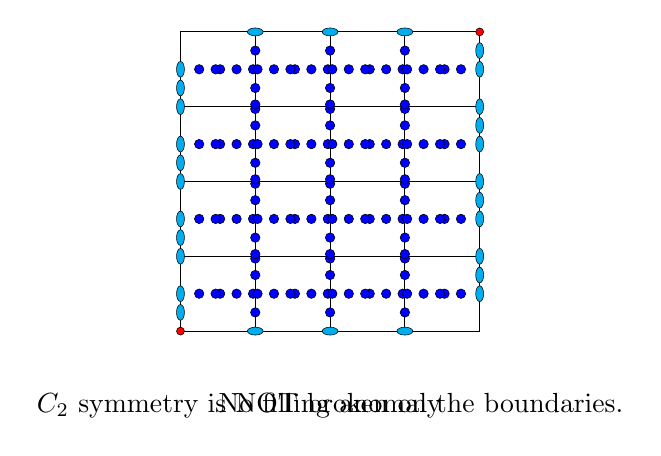
\begin{tikzpicture}[scale = 0.95]
            \draw[black] (0,0) grid(4,4);
    
            \foreach \i in {0,...,3} 
            \foreach \j in {0,...,3} 
            {
            \draw[black] (\i+0.45,\j+0.45) -- (\i+0.55,\j+0.55);
            \draw[black] (\i+0.45,\j+0.55) -- (\i+0.55,\j+0.45);
            }
            \visible<1>{
            \foreach \i in {0,...,3} 
            \foreach \j in {0,...,3} 
            {
            \draw[fill=blue, very thin] (\i+0.03+0.5 ,\j+0.5) circle (1.8pt);
            \draw[fill=blue, very thin] (\i-0.03+0.5 ,\j+0.5) circle (1.8pt);
            }
            }
            \visible<2>{
            \foreach \i in {0,...,3} 
            \foreach \j in {0,...,3} 
            {
            \draw[fill=blue, very thin] (\i+0.5+0.25 ,\j+0.5) circle (1.8pt);
            \draw[fill=blue, very thin] (\i+0.5-0.25 ,\j+0.5) circle (1.8pt);
            }
            }
            \visible<3>{
            \foreach \j in {0,...,3} 
            {
            \foreach \i in {0,...,2} 
            {
            \draw[fill=blue, very thin] (\i+0.97 ,\j+0.5) circle (1.8pt);
            }
            \draw[fill=cyan, very thin] (4, \j+0.5) ellipse (1.5pt and 3pt);
            }
            \foreach \j in {0,...,3} 
            {
            \foreach \i in {1,...,3} 
            {
            \draw[fill=blue, very thin] (\i+0.03 ,\j+0.5) circle (1.8pt);
            }
            \draw[fill=cyan, very thin] (0, \j+0.5) ellipse (1.5pt and 3pt);
            }
            }
        
            \visible<4>{
            \foreach \j in {0,...,3}
            { 
            \foreach \i in {1,...,3} 
            {
            \draw[fill=blue, very thin] (\i ,\j+0.5-0.25) circle (1.8pt);
            }
            \draw[fill=cyan, very thin] (0, \j+0.5-0.25) ellipse (1.5pt and 3pt);
            }
            \foreach \j in {0,...,3}
            { 
            \foreach \i in {0,...,2} 
            {
            \draw[fill=blue, very thin] (\i+1 ,\j+0.5+0.25) circle (1.8pt);
            }
            \draw[fill=cyan, very thin] (4, \j+0.5+0.25) ellipse (1.5pt and 3pt);
            }
            \node[align=center] at (2,-1) {$C_2$ symmetry is NOT broken on the boundaries.};
            }
            \visible<5>{
            \foreach \j in {0,...,2} 
            \foreach \i in {0,...,2} 
            {
            \draw[fill=blue, very thin] (\i+1 ,\j+0.97) circle (1.8pt);
            \draw[fill=blue, very thin] (\i+1 ,\j+1.03) circle (1.8pt);
            }
            \foreach \j in {0,...,2}
            {
            \draw[fill=cyan, very thin] (0, \j+1) ellipse (1.5pt and 3pt);
            \draw[fill=cyan, very thin] (4, \j+1) ellipse (1.5pt and 3pt);
            }
            \foreach \i in {0,...,2}
            {
            \draw[fill=cyan, very thin] (\i+1, 4) ellipse (3pt and 1.5pt);
            \draw[fill=cyan, very thin] (\i+1, 0) ellipse (3pt and 1.5pt);
            }
            \draw[fill=red, very thin] (0 ,0) circle (1.5pt);
            \draw[fill=red, very thin] (4 ,4) circle (1.5pt);
            \node[align=center] at (2,-1) {No filling anomaly};
            }
        \end{tikzpicture}%
        }
    \end{figure}
\end{frame}

\begin{frame}
    \frametitle{Boundary obstructed atomic phases.} 
    Boundary obstruction protected by $C_2$ and $\mathcal{P}$ symmetry: 
    \begin{figure}[]
        \subfigure{
        \centering
        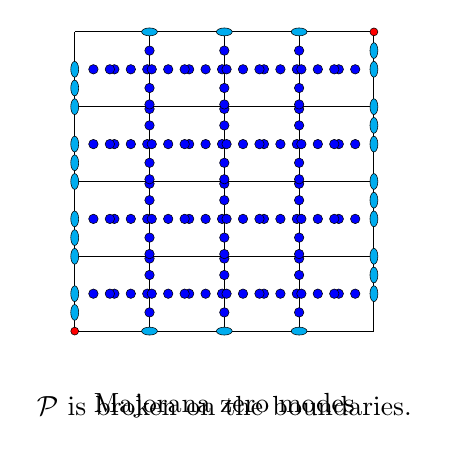
\begin{tikzpicture}[scale = 0.95]
            \draw[black] (0,0) grid(4,4);
    
            \foreach \i in {0,...,3} 
            \foreach \j in {0,...,3} 
            {
            \draw[black] (\i+0.45,\j+0.45) -- (\i+0.55,\j+0.55);
            \draw[black] (\i+0.45,\j+0.55) -- (\i+0.55,\j+0.45);
            }
            \visible<1>{
            \foreach \i in {0,...,3} 
            \foreach \j in {0,...,3} 
            {
            \draw[fill=blue, very thin] (\i+0.03+0.5 ,\j+0.5) circle (1.8pt);
            \draw[fill=blue, very thin] (\i-0.03+0.5 ,\j+0.5) circle (1.8pt);
            }
            }
            \visible<2>{
            \foreach \i in {0,...,3} 
            \foreach \j in {0,...,3} 
            {
            \draw[fill=blue, very thin] (\i+0.5+0.25 ,\j+0.5) circle (1.8pt);
            \draw[fill=blue, very thin] (\i+0.5-0.25 ,\j+0.5) circle (1.8pt);
            }
            }
            \visible<3>{
            \foreach \j in {0,...,3} 
            {
            \foreach \i in {0,...,2} 
            {
            \draw[fill=blue, very thin] (\i+0.97 ,\j+0.5) circle (1.8pt);
            }
            \draw[fill=cyan, very thin] (4, \j+0.5) ellipse (1.5pt and 3pt);
            }
            \foreach \j in {0,...,3} 
            {
            \foreach \i in {1,...,3} 
            {
            \draw[fill=blue, very thin] (\i+0.03 ,\j+0.5) circle (1.8pt);
            }
            \draw[fill=cyan, very thin] (0, \j+0.5) ellipse (1.5pt and 3pt);
            }
            }
        
            \visible<4>{
            \foreach \j in {0,...,3}
            { 
            \foreach \i in {1,...,3} 
            {
            \draw[fill=blue, very thin] (\i ,\j+0.5-0.25) circle (1.8pt);
            }
            \draw[fill=cyan, very thin] (0, \j+0.5-0.25) ellipse (1.5pt and 3pt);
            }
            \foreach \j in {0,...,3}
            { 
            \foreach \i in {0,...,2} 
            {
            \draw[fill=blue, very thin] (\i+1 ,\j+0.5+0.25) circle (1.8pt);
            }
            \draw[fill=cyan, very thin] (4, \j+0.5+0.25) ellipse (1.5pt and 3pt);
            }
            \node[align=center] at (2,-1) {$\mathcal{P}$ is broken on the boundaries.};
            }
            \visible<5>{
            \foreach \j in {0,...,2} 
            \foreach \i in {0,...,2} 
            {
            \draw[fill=blue, very thin] (\i+1 ,\j+0.97) circle (1.8pt);
            \draw[fill=blue, very thin] (\i+1 ,\j+1.03) circle (1.8pt);
            }
            \foreach \j in {0,...,2}
            {
            \draw[fill=cyan, very thin] (0, \j+1) ellipse (1.5pt and 3pt);
            \draw[fill=cyan, very thin] (4, \j+1) ellipse (1.5pt and 3pt);
            }
            \foreach \i in {0,...,2}
            {
            \draw[fill=cyan, very thin] (\i+1, 4) ellipse (3pt and 1.5pt);
            \draw[fill=cyan, very thin] (\i+1, 0) ellipse (3pt and 1.5pt);
            }
            \draw[fill=red, very thin] (0 ,0) circle (1.5pt);
            \draw[fill=red, very thin] (4 ,4) circle (1.5pt);
            \node[align=center] at (2,-1) {Majorana zero modes};
            }
        \end{tikzpicture}%
        }
    \end{figure}
\end{frame}

\begin{frame}
    \frametitle{Boundary obstructed atomic phases.}

    \begin{columns}
        \begin{column}{0.5\textwidth}
                \begin{table}
                    \centering
                    \def\arraystretch{0.4}
                    \begin{adjustbox}{width=\columnwidth,center}
                        \begin{tabular}{|| p{2.5cm}| p{2.5cm} | p{2.5cm}||} 
                        \hline
                        \begin{center} Model \end{center} 
                        &  \begin{center} With $C_{4}$ \end{center}   & \begin{center} With $C_{2}$  \end{center} \\ 
                        \hline\hline
                        \begin{center}
                        With PH
                        \end{center}
                        & %\rule{0pt}{4.6ex}
                        \begin{center}
                        HOTSC$_{2}$; \\
                        %\newline with 
                        corner Majorana 
                        %{\rule[-3.2ex]{0pt}{0pt}} 
                        \end{center}
                        & 
                        \begin{center}
                        BOTSC$_2$; \\
                        %\newline with 
                        corner Majorana 
                        \end{center}
                        \\ 
                        \hline
                        \begin{center}
                        Without PH
                        \end{center} &
                        \begin{center}
                        HOTI$_{2}$; \\
                        %\rule{0pt}{4.6ex}
                        % \newline with 
                        filling anomaly
                        % {\rule[-3.2ex]{0pt}{0pt}}
                        \end{center}
                        & 
                        \begin{center}
                        Trivial
                        \end{center}
                            \\ 
                        \hline
                        \end{tabular}
                \end{adjustbox}
            \end{table}
        \end{column}
        \begin{column}{0.5\textwidth}
            \begin{itemize}
                \item Atomic phases show the importance of particle-hole symmetry to protect the boundary obstructed phase.  \pause 
                \item Next we show explicitly that our 'Dirac + ($p+ip)$' model with $C_2$ symmetry is indeed boundary obstructed, by studying its edge theory. 
            \end{itemize}
        \end{column}
    \end{columns}


\end{frame}

\begin{frame}
    \frametitle{Interlude: The Wannier bands}
    Loosely, the Wannier Hamiltonian is a bulk defined object that has a spectrum that is smoothly connected to that of the edges. \pause
    
    Wannier Hamiltonian is defined using Wilson loops as: 
    \begin{columns}
        \begin{column}{0.8\textwidth}
            \begin{align*}
                &\hat\nu^{mn}_y(k_x) \equiv \frac{1}{2\pi i} \oint dk_y \braket{u^m(k_x,k_y)|\partial_{k_y}u^n(k_x,k_y)} \nonumber \\ 
                &\ket{u^{m}(\bm k )} \ \text{are the occupied states of the Hamiltonian.}
            \end{align*}
        \end{column}
        \begin{column}{0.2\textwidth}
            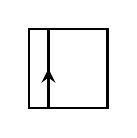
\begin{tikzpicture}[scale=0.5]
                \draw[black, thick] (-1,-1) rectangle (1,1);
                \draw[black, very thick, postaction={on each segment={mid arrow=black}}] (-0.5,-1) -- (-0.5,1);
            \end{tikzpicture}
        \end{column}
    \end{columns}\pause
    \begin{figure}[]
        \centering
        \subfigure{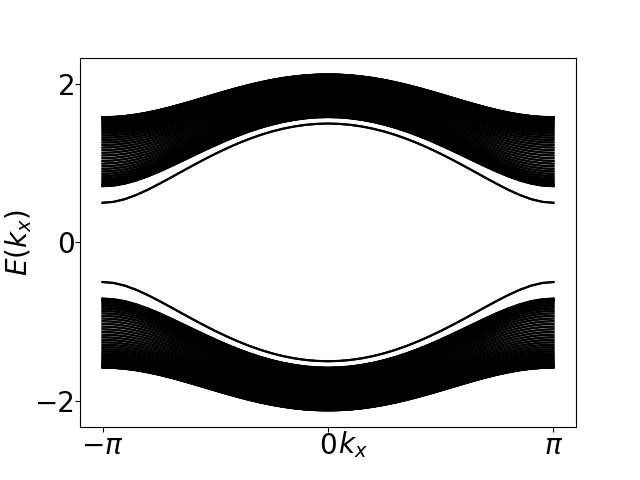
\includegraphics[scale=0.3]{energy_cylinder.png}}
        \subfigure{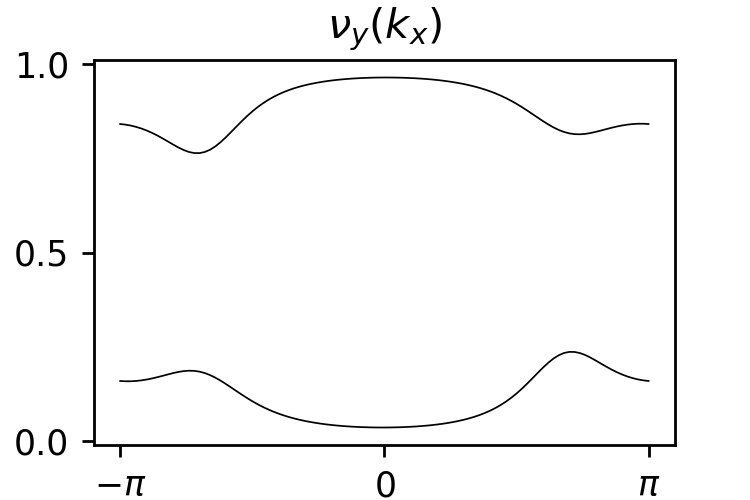
\includegraphics[scale=0.7]{wannier_bands_demo.png}}
    \end{figure}

\end{frame}

\begin{frame}
    \frametitle{Wannier bands detect boundary gap closing.}
    \framesubtitle{A relative bulk topological invariant}
    \begin{align*}
        H= & (\cos k_x+ \gamma_x) \sigma_x\tau_z +  \cos k_y  \sigma_z\tau_z - 0.2 \tau_z \nonumber\\
        &+ 0.4 \sin k_x \tau_x + 0.4 \sin k_y \tau_y
    \end{align*}
    \begin{figure}[t]
        \centering
        \subfigure{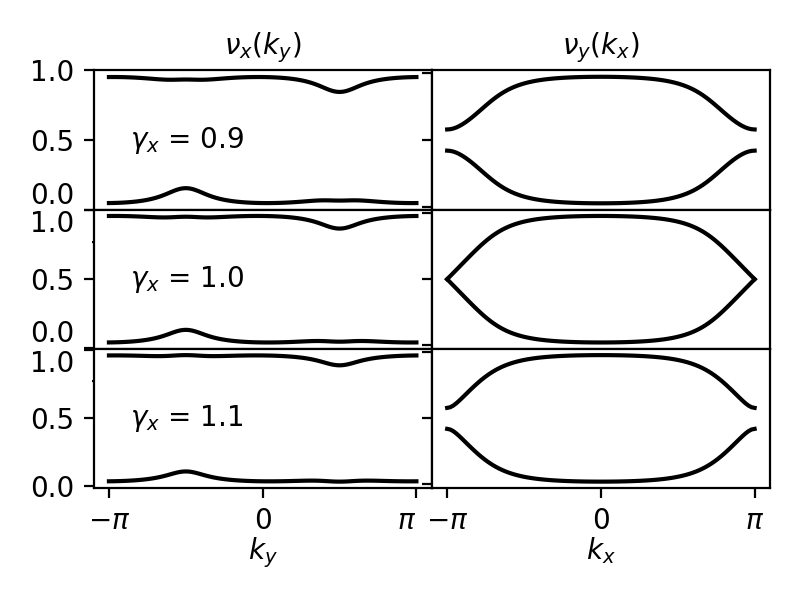
\includegraphics[trim= 0 10 0 0, clip,scale=0.45]{wannier_spec_gamma_array_x.png}}
        \subfigure{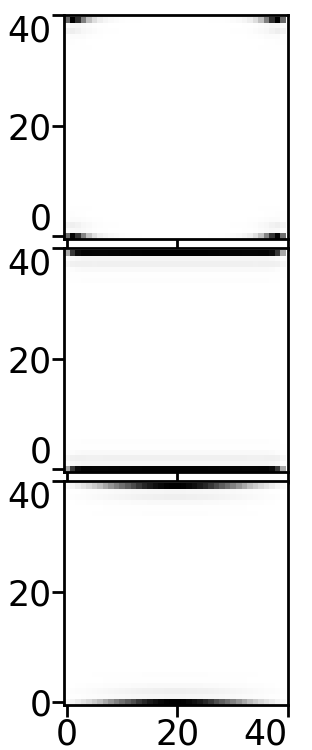
\includegraphics[scale=0.425]{corner_modes_gamma_x_array.png}}
        \subfigure{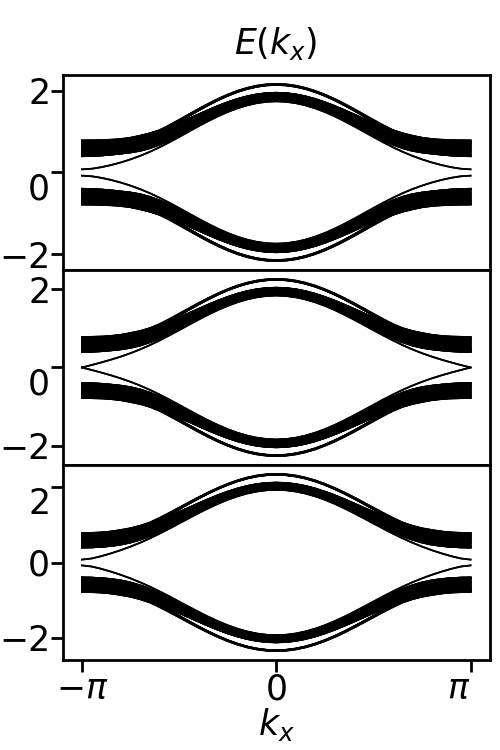
\includegraphics[scale=0.45]{spectrum_cylinder_gamma_array.png}}
    \end{figure}
    \begin{itemize}
        \item That the Wannier bands gap closing, being a property of the bulk, can be used to define some bulk topological invariant.However the exact form of that invariant may be complicated. 
    \end{itemize} 
\end{frame}

\begin{frame}
    \frametitle{Wannier-projected Hamiltonian}
    \begin{align*}
        H_{P^\pm}(k_x)=&P^\pm (k_x) H P^\pm (k_x)
        , \textrm{where} \\ 
        P^\pm (k_x)\equiv&\frac{1\pm\hat P_{\rm occ}(\bm k)\sgn(\hat \nu_y)\pm\hat P_{\rm emp}(\bm k)\sgn(\hat \nu_y')}{2} \\
        \tilde{\mathcal{P}}(k_x) K =& P^\pm ( k_x)\mathcal{P} \[P^{\pm}(- k_x)\]^* K \nonumber\\ 
        H_{P^\pm}(k_x) =& - {\tilde{\mathcal{P}}}(k_x) H^*_{P^\pm}(-k_x) {\tilde{\mathcal{P}}}^\dagger(k_x)
    \end{align*}\pause
    We use $H_{P^\pm}(k_x=0,\pi)$ as a zero dimensional subsystems. 
    \begin{overpic}[width=\textwidth]{defect_classification.png}
        \put (47.5,14.2) 
        {
            
\begin{tikzpicture}
                \draw[red, thick] (0,0) circle (5pt);
            \end{tikzpicture}
        }
    \end{overpic}

\end{frame}

\begin{frame}
    \frametitle{A recipie for getting edge Hamiltonian}
    \begin{columns}
        \begin{column}{0.7\textwidth}
            \begin{enumerate}
                \visible<1->{
                \item Choose a direction, $\theta$, to put the edge. }
                \visible<2->{
                \item Choose how you model empty space. (Different choices will lead to different boundary conditions but doesn't change the physics of the boundary.) $\mathcal{H}(\bm k) \rightarrow \mathcal{H}(\partial_{x_\perp},k_{||},x_\perp)$ }
                \visible<3->{
                \item Solve for the localized edge states. $\Psi_{\alpha}^{\text{edge}}(x_\perp,k_{||}) = e^{ik_{||} x_{||}} \chi_{\alpha}(k_{||}) \phi(x_{\perp})$, such that, $\mathcal{H} \Psi_{\alpha}^{\text{edge}} = \epsilon^{\alpha}(k_{||}) \Psi_{\alpha}^{\text{edge}}$ }
                \visible<4->{
                \item The edge Hamiltonian is then, $h^{\text{edge}}(k_{||}) = \sum_{\alpha} \ket{\chi_{\alpha}(k_{||})} \epsilon^{\alpha}(k_{||}) \bra{\chi_{\alpha}(k_{||})}$}
            \end{enumerate}
        \end{column}
        \begin{column}{0.3\textwidth}
            \visible<1->{
            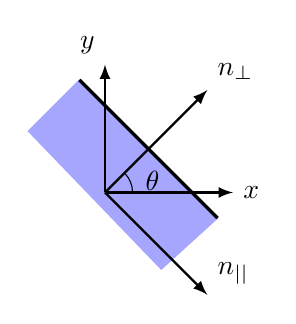
\begin{tikzpicture}[scale=0.65]
                \draw[fill,blue!35] (-0.5,2.2) -- (2.2,-0.5) -- (1.1,-1.5) -- (-1.5,1.2) -- cycle;
                \draw[very thick] (-0.5,2.2) -- (2.2,-0.5);
                \draw[thick,->] (0,0) -- (2.5,0) node[anchor=west] (x) {$x$};
                \draw[thick,->] (0,0) -- (0,2.5) node[anchor=south east] (y) {$y$};
                \draw[thick,->] (0,0) -- (2,2) node[anchor=south west] (n){$n_{\perp}$};
                \draw[thick,->] (0,0) -- (2,-2) node[anchor=south west]{$n_{||}$};
                \node (o) at (0,0) {};
                \draw pic["$\theta$",draw=black,angle eccentricity=1.2,anchor=west,angle radius=0.35cm] {angle=x--o--n};
            \end{tikzpicture}
            }
        \end{column}
    \end{columns}
\end{frame}

\begin{frame}
    \frametitle{Majorana zero modes as a defect of the edge}
    \begin{columns}
        \begin{column}{0.55\textwidth}
            \begin{align*}
                &\mathcal{H}(\bm k) = f_1 (\bm k) \sigma_x\tau_z + f_2(\bm k) \sigma_z\tau_z  \\
                & \qquad + \epsilon g_1(\bm k) \tau_x + \epsilon g_2(\bm k) \tau_y - \mu\tau_z \\ 
                &k_x(\theta)=k_\perp \cos\theta - k_\| \sin\theta \nonumber\\
                &k_y(\theta)=k_\perp \sin\theta + k_\| \cos\theta \\
                &H\to \tilde H= UHU^\dagger \\ 
                \end{align*}
        \end{column}
        \begin{column}{0.45\textwidth}
            \begin{figure}[]
                \centering
                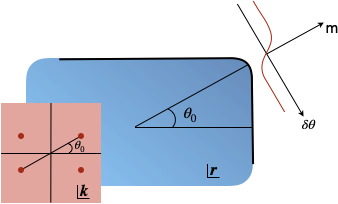
\includegraphics[scale=0.35]{corner_without_C4.png}
            \end{figure}
        \end{column}
    \end{columns}
    \begin{align*}
        \tilde H(k_\perp,k_\|=0;\theta_0)=\tilde f_1(k_\perp)  \sigma_x\tau_z  + \epsilon \tilde g_1(k_\perp) \tau_x  - \mu\tau_z 
    \end{align*}
    Do a perturbative expansion for: 
    (i)  Small $k_\| $, 
    (ii) Small $\delta \theta$
    \begin{align*}
        h(k_{\|}, \theta_0+\delta\theta) = \alpha k_\| s_x + \beta \delta\theta s_y.
    \end{align*}
    \begin{itemize}
        \item This looks like a kitaev chain with a domain wall, hence it host a Majorana zero mode. 
    \end{itemize}
\end{frame}

\begin{frame}
    \frametitle{Summary}

    \begin{table}
        \centering
        \def\arraystretch{0.4}
         \begin{tabular}{|| p{2.5cm}| p{2.5cm} | p{2.5cm}||} 
         \hline
         \begin{center} Model \end{center} 
          &  \begin{center} With $\ms{C}_{4}$ \end{center}   & \begin{center} With $\ms{C}_{2}$  \end{center} \\ 
         \hline\hline
         \begin{center}
        With PH
        \end{center}
        & %\rule{0pt}{4.6ex}
        \begin{center}
        HOTSC$_{2}$; \\
        %\newline with 
        corner Majorana 
        %{\rule[-3.2ex]{0pt}{0pt}} 
        \end{center}
        & 
        \begin{center}
        BOTSC$_2$; \\
        %\newline with 
        corner Majorana 
        \end{center}
        \\ 
          \hline
         \begin{center}
         Without PH
          \end{center} &
         \begin{center}
         HOTI$_{2}$; \\
         %\rule{0pt}{4.6ex}
        % \newline with 
         filling anomaly
        % {\rule[-3.2ex]{0pt}{0pt}}
         \end{center}
          & 
          \begin{center}
          Trivial
          \end{center}
             \\ 
          \hline
        \end{tabular}
    \end{table}

\end{frame}
\end{document}
